\documentclass[border=5pt]{standalone}
\usepackage{tikz}
\usetikzlibrary{decorations.markings}
\usepackage{amsmath, amssymb}

\begin{document}

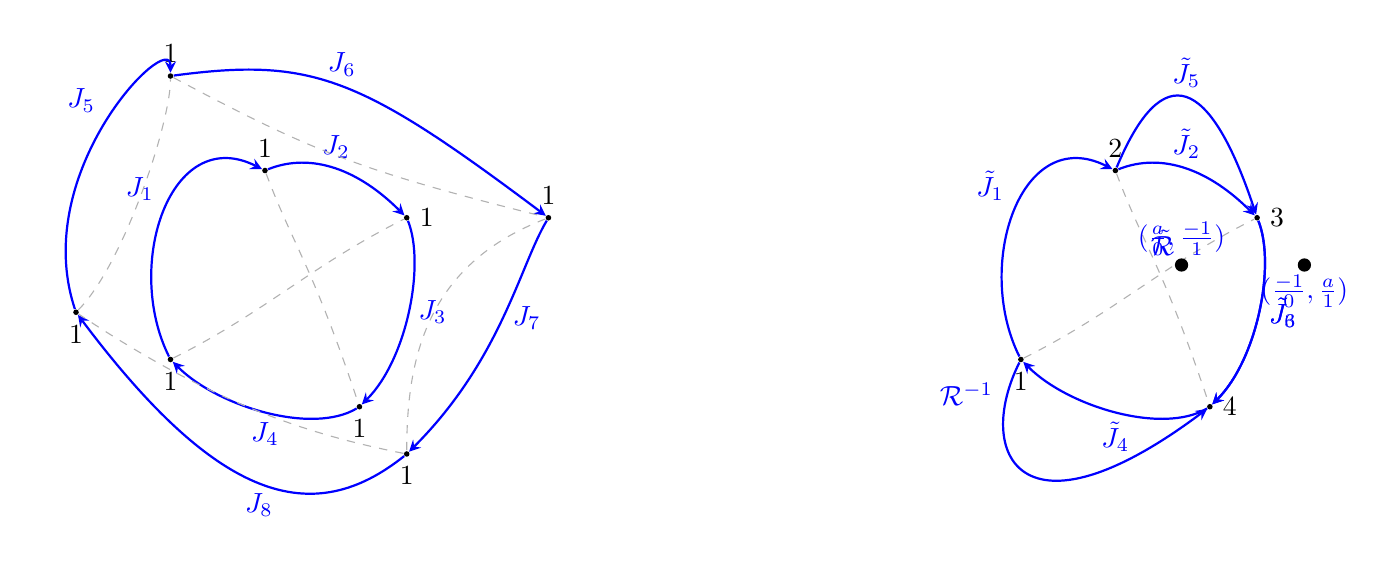
\begin{tikzpicture}[scale=1.2]

% 定义样式
\tikzset{
  point/.style={circle, fill, minimum size=2pt, inner sep=0pt},
  hollow point/.style={circle, draw, minimum size=2pt, inner sep=0pt},
  blue curve/.style={blue, thick, ->, >=stealth},
  gray curve/.style={gray!60, dashed}
}

% 左侧图形
\begin{scope}[shift={(-6,0)}]
  % 点
  \node[point, label={below:$1$}] (p1) at (-1.5,-1) {};
  \node[point, label={above:$1$}] (p2) at (-0.5,1) {};
  \node[point, label={right:$1$}] (p3) at (1,0.5) {};
  \node[point, label={below:$1$}] (p4) at (0.5,-1.5) {};
  \node[point, label={below:$1$}] (p5) at (-2.5,-0.5) {};
  \node[point, label={above:$1$}] (p6) at (-1.5,2) {};
  \node[point, label={above:$1$}] (p7) at (2.5,0.5) {};
  \node[point, label={below:$1$}] (p8) at (1,-2) {};

  % 蓝色曲线
  \draw[blue curve] (p1) .. controls (-2,0) and (-1.5,1.5) .. (p2) node[midway, above left] {$J_1$};
  \draw[blue curve] (p2) .. controls (0,1.2) and (0.5,1) .. (p3) node[midway, above] {$J_2$};
  \draw[blue curve] (p3) .. controls (1.2,0) and (1,-1) .. (p4) node[midway, right] {$J_3$};
  \draw[blue curve] (p4) .. controls (0,-1.8) and (-1,-1.5) .. (p1) node[midway, below] {$J_4$};
  \draw[blue curve] (p5) .. controls (-3,1) and (-1.5,2.5) .. (p6) node[midway, above left] {$J_5$};
  \draw[blue curve] (p6) .. controls (0,2.2) and (0.5,2) .. (p7) node[midway, above] {$J_6$};
  \draw[blue curve] (p7) .. controls (2.2,0) and (2,-1) .. (p8) node[midway, right] {$J_7$};
  \draw[blue curve] (p8) .. controls (0,-2.8) and (-1,-2.5) .. (p5) node[midway, below] {$J_8$};

  % 灰色虚线
  \draw[gray curve] (p1) .. controls (-0.5,-0.5) and (0,0) .. (p3);
  \draw[gray curve] (p2) .. controls (-0.2,0.2) and (0,0) .. (p4);
  \draw[gray curve] (p5) .. controls (-2,0) and (-1.5,1.5) .. (p6);
  \draw[gray curve] (p6) .. controls (0,1.2) and (0.5,1) .. (p7);
  \draw[gray curve] (p7) .. controls (1.2,0) and (1,-1) .. (p8);
  \draw[gray curve] (p8) .. controls (0,-1.8) and (-1,-1.5) .. (p5);
\end{scope}

% 右侧图形
\begin{scope}[shift={(3,0)}]
  % 点
  \node[point, label={below:$1$}] (p1) at (-1.5,-1) {};
  \node[point, label={above:$2$}] (p2) at (-0.5,1) {};
  \node[point, label={right:$3$}] (p3) at (1,0.5) {};
  \node[point, label={right:$4$}] (p4) at (0.5,-1.5) {};
  \node[point] (p5) at (0.2,0) {};
  \node[hollow point] (p6) at (1.5,0) {};
  
  % 蓝色曲线
  \draw[blue curve] (p1) .. controls (-2,0) and (-1.5,1.5) .. (p2) node[midway, above left] {$\tilde{J}_1$};
  \draw[blue curve] (p2) .. controls (0,1.2) and (0.5,1) .. (p3) node[midway, above] {$\tilde{J}_2$};
  \draw[blue curve] (p3) .. controls (1.2,0) and (1,-1) .. (p4) node[midway, right] {$\tilde{J}_3$};
  \draw[blue curve] (p4) .. controls (0,-1.8) and (-1,-1.5) .. (p1) node[midway, below] {$\tilde{J}_4$};
  \draw[blue curve] (p1) .. controls (-2,-2) and (-1.5,-3) .. (p4) node[pos=0.2, above left] {$\mathcal{R}^{-1}$};
  \draw[blue curve] (p2) .. controls (0,2.2) and (0.5,2) .. (p3) node[midway, above] {$\tilde{J}_5$};
  \draw[blue curve] (p3) .. controls (1.2,0) and (1,-1) .. (p4) node[midway, right] {$\tilde{J}_6$};

  % 灰色虚线
  \draw[gray curve] (p1) .. controls (-0.5,-0.5) and (0,0) .. (p3);
  \draw[gray curve] (p2) .. controls (-0.2,0.2) and (0,0) .. (p4);

  % 点标记
  \node[blue] at (p5) [above] {$(\frac{a}{0}, \frac{-1}{1})$};
  \node[blue] at (p6) [below] {$(\frac{-1}{0}, \frac{a}{1})$};
  \node[blue] at (0,0) [above] {$\tilde{\mathcal{R}}$};
  
  % 中心点标记
  \fill[black] (p5) circle (2pt);
  \fill[black] (p6) circle (2pt);
\end{scope}

\end{tikzpicture}

\end{document}